\chapter{Foundations}
\section{Model-Driven Software Development}
Due to the increasing complexity of software-based systems, the abstraction level of software has to be increased. Model-driven software development (MDSD) is a software development method which focuses on creating abstract models with a strong inner structure. Traditional ways of software development have exhibited difficulties to maintain and grant stability in their structure, due to the fact programming languages do meet their limitations very quickly, when it comes to abstraction. Models are still present in the traditional approaches for documentation purpose and to prevent inconsistency. However, its structure is hardly recognizable after the development process. The model driven approach present more efficiency, and disengages from the model based approach. Since models are constructed in a formal and abstract manner, they can abstract the software's source code completely. Hence, the inner structure of an artefact can be made compact and lucid, even for a person with no prior programming knowledge \cite{voelter2007product}.
The model is the development's primary source and is also considered being part of the final implementation. The architecture a system should have as well as the functionality it should provide can be stated in a model. Hence, there is no need for the developers to impart every detail about the software implementation to the end-user any more. Despite the fact that the software development industry is experiencing a dramatic change, of the way applications are implemented, there is no accurate definition for MDSD's specifications. However, there are still some requirements that can be implicated\cite{AtkinsonG16}. Due to the significant motivation companies, that use MDSD have, to enhance productivity, raising the return on investment of their products became a crucial factor. A company can benefit from this, whether through improving the developers' productivity in the short run, by extending a relevant software artefact's functionality, or by improving their productivity in the long run, by investing into software that is long living. Most of the companies using this approach choose the former one, and tend to enhance the functionality of an already available artefact. Hence, "the more executable functionality it can generate, the higher the productivity will be"\cite{AtkinsonG16}. The second approach is less common, although the higher the longevity of an artefact is, the more the return on investment increases. Therefore, a decreasing sensitivity for change of an institution's main artefacts is desirable. From the MDSD point of view this even forms a requirement for it.
Nowadays automated code generation enhances software quality and devlopement speed, and parts of the code can be reusable components after their definition.
Recent studies show that the influences on quality, performance, and time may depend on whether a general purpose language, or a domain-specific language was used to implement the development process. The successful application of model-driven development was significantly higher in case of a domain-specific language (DSL)\cite{whittle2014state}. Therefore, it is recommended to use MDSD with ontological modeling.\\
Due to games being software from a technical point of view, all relevant requirements and characteristics from MDSD can be applied to model-driven game development as well.
\section{Deep Modelling}
\begin{figure}
	\centering
	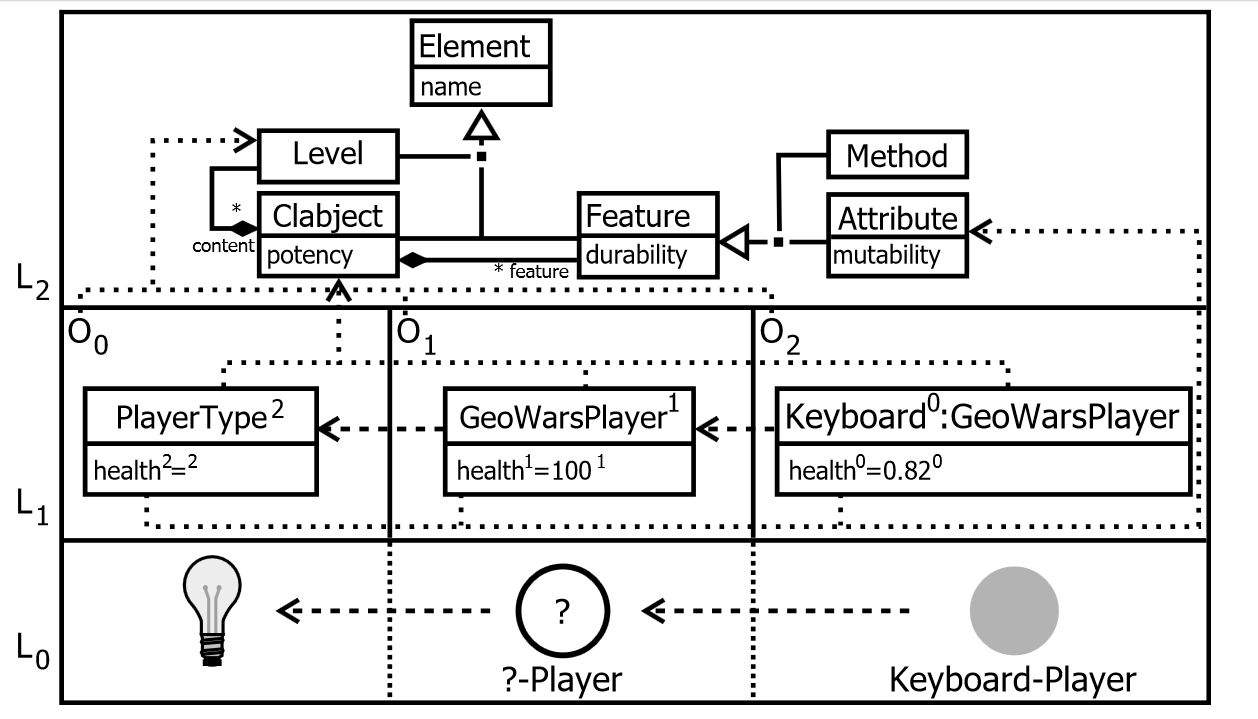
\includegraphics[scale=0.25]{grafiken/OCA.jpg} 
	\caption{The Orthogonal Classification Architecture\cite{exe2015}}
	\label{fig:1}
\end{figure}
Deep Modelling is a multi-level modelling technique developed by Atkinson and Kuehne to support model-driven software development. Conventional modelling languages and tools are based on the traditional "two levels": first the type level, in which the modelling language is described, and second the instance level containing the user model. This "two level" approach entails certain limitations, due to the lacking space for modelling instances of the user model \cite{AtkinsonG16} Deep modeling differs from this by allowing more than one logical class/instance level for a chosen domain. It supports creating models with an arbitrary number of classification levels, based on the Orthogonal Classification Architecture (OCA). Two kinds of classification relationships can be observed in [Fig. \ref{fig:1}], which illustrates an extract from the deep model of GeoWars, a multi-level model based Simulation developed by the chair of software engineering in Mannheim. The vertical dimension represents the linguistic stack, which describes all relevant concepts available in multi-level-modelling languages and entails all ontological levels. It represents the Object Management Group's Model-Driven-Architecture-Modeling-Stack\cite{AtkinsonG16}. 
The horizontal dimension describes the ontological levels.\\ L2 represents all model elements. It is referred to as the "linguistic (meta) model". The middle level L1 consists of content of the regarded domain. Thus, it holds the actual deep model and its ontological levels, O0 to O2. All model elements in L1, those in O0 excluded, each have a linguistic and a ontological type.  The lowest level (L0), consists of the real world entities, which are part of the ontological content of L1. At least three levels are typically required for model simulation and for the execution of a domain. In general the first level O0 defines the modelling language, O1 describes the model of the domain, and the third level O2 describes the instances of our domain objects, and with this the execution state of our model. Due to the fact that model elements of O1 represent instances of the types from the ontological level above and further represent types for the instances in the level underneath, they are referred to as \textit{Clabjects}, a word derived from "Class" and "Object".
Although this three level composition has become prevalent, the number of levels is unlimited in general. By deep instantiation the number of consecutive levels in which an entity from the model can be instantiated is determined. Furthermore it describes how deep a certain type can influence other types.

\section{The Eclipse Project and PDE}
The Eclipse Project is an open source software development project, which allows the development and provision of highly integrated tools.
A generic core framework for tool integration is provided, which is used by a Java development environment built. The Eclipse kernel contains a plug-in loader, which is gridded with an arbitrary amount of plug-ins. Plug-ins in the Eclipse context, are not plug-ins in the traditional way. They rather connect with a universe of plug-ins to form a running system. By being executed in an environment provided by this kernel, they can extend the environment’s services, by adding extension point to the system. Other plug-ins relying on these services can add them as an extension, to use these services. Due to the Eclipse Project's modular design, users can develop and install additional plug-ins into their workbench to extend its functionality. For developing plug-ins, the Plug-in Development Environment (PDE) is provided. It is a subproject of the Eclipse Project, which provides several tools for creating, developing, testing, debugging, building and deploying Eclipse plug-ins, fragments, features, update sites and RCP.
\section{Eclipse Modeling Framework}
The Eclipse Modeling Framework (EMF) is a code generation facility for Eclipse. It brings together the high- level engineering and modelling work and the low-level implementation programming, as two well-integrated parts of the same work. EMF provides building tools and other applications that enable the definition of a meta-metamodel from the actual model, also referred to as ecore-model. The ecore-model entails the defined classes and their names, attributes and methods. A genmodel can then be generated from the defined ecore model, which is considered to be the meta-model of our model. Afterwards the genmodel is used for describing instances of the classes from our ecore-model. Subsequently, it allows creating the domain model and the Java implementation of the meta-model, consisting the relevant instances and their attributes. Changes in a model from a higher level are forwarded to all lower level representations, due to the connection the different modelling levels have. Due to the fact that modelling concepts being directly related to their implementation, EMF allows modelling with a low cost of entry
Hence, an EMF model connects the main technologies, Java, XML, and UML, and regardless of which technology is used to define it, an EMF model is the common high-level representation that glues them all together. Therefore, it is not surprising that EMF has become a model driven software development standard, and is widely used in the industry.

\section{Graphical Modeling Framework}
The Graphical Modeling Framework(GMF) is a framework for implementing graphical editors based on EMF and GEF. For this purpose it provides certain features, like a set of reusable graphical components, a model enabling the description of diagram elements and distinguishes between the semantic (domain) and notation (diagram) elements. Moreover it provides a command infrastructure which bypasses the distinct parts of EMF's and GEF's command frameworks. Furthermore GMF is extensible and allows the implemented editors to be open and extensible.

\section{Melanee}
\begin{figure}
	\centering
	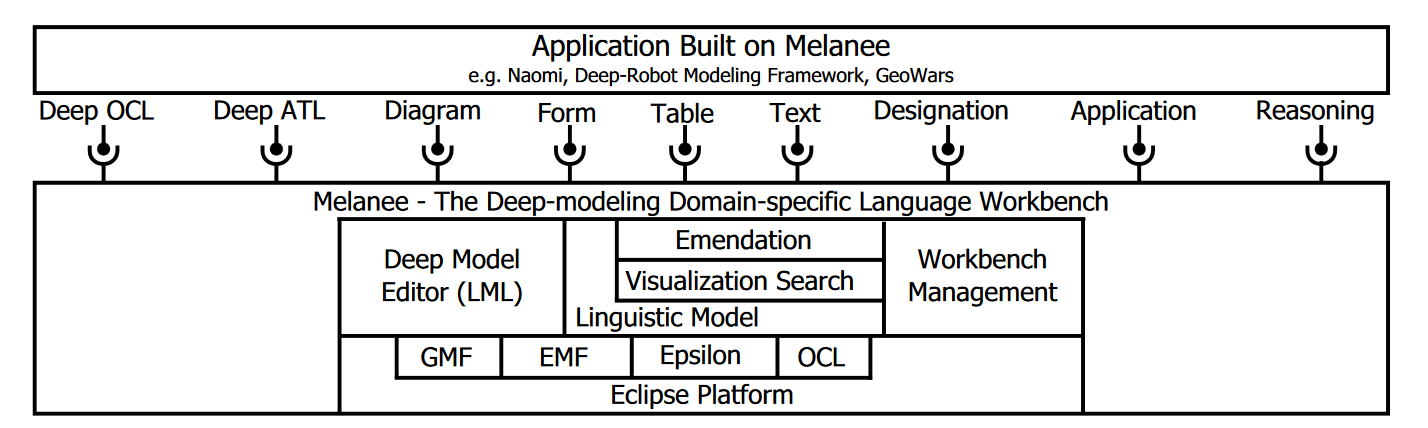
\includegraphics[width=425pt]{grafiken/extensionPoint.png}
	\caption{Melanee Architecture\cite{AtkinsonG16}}
	\label{fig:2}
\end{figure}
Melanee, developed by the Software Engineering Group at the University of Mannheim, is a workbench for creating domain-specific languages. It is based on the OCA principles and occupies an arbitrary number of ontological levels. \cite{MEL}  Most modelling tools focus on one specific format for creating domain specific languages and are regularly limited to support just two classification levels. As opposed to this Melanee supports multi-format, multi-notation domain specific modelling and due to its extendable structure the formats are limitless. The Eclipse frameworks GMF and EMF are integrated into Melanee's workbench and moreover form its foundation. This enables the use of a variety of EMF-languages and tools, which allow the deep modelling approach. Due to the fact that Melanee is an Eclipse-based application, its functionality can be extended by developing plug-ins with the Eclipse PDE. By developing extension points the contributed functionalities can be integrated into the workbench. Already available extension points, like the Deep OCL constraint language, the Deep ATL transformation language, which enables the transformation of a deep model into an ecore model, vice versa, and deep model to deep model transformation, an application language which provides altering the model environment, Reasoning, which includes model checking, and a few DSL extensions, intended to put predefined and user-defined DSLs, into the corresponding formats. Melanee is partitioned in separable components, which can be observed in [Fig. \ref{fig:2}]. The included figure shows the architecture of Melanee. It's core application offers the following features: the linguistic model, the deep model editor, visualization search algorithm, the emendation service and workbench management functionality \cite{AtkinsonG16}.

\subsection{The Level-agnostic Modeling Language and its Editor}
Creating Deep Models and defining ontological levels in it is enabled in Melanee by using the Level-agnostic Modelling language (LML). It is provided as an Eclipse plug-in, but can also be deployed as an Eclipse RCP application. %\cite{RalphDis} 
Deep instantiation is implemented in Melanee through potency attached to Clabjects (potency), Features (durability), and Attribute values (mutability)\cite{exe2015}. If an entity is defined its default potency is set to 1. When a Clabject is instantiated in a level above, its potency is decremented. If the potency of a Clabject reaches 0, it can not be instantiated in a level above.In the first level "O0" the modelling language can be specified by adding “Entities”, “Attributes”, “Methods”, “Connections/Roles”, etc. In all consecutive levels additional entities can be defined, and the entities defined in a prior level can be instantiated. 


\subsection{Extension Points and Extensions}
Since Melanee is an Eclipse based Application, the Eclipse concept of Extensions and Extension Points can be used to contribute functionality to the Melanee API. An Eclipse plug-in can use existing Extension Points as an Extension, or define Extension Points, so other plug-ins can use them as Extension. org.melanee.core.popupbutton.provider is a Melanee Extension Point of its workbench plug-in. Other Melanee pugins, which set it as an extension, can use the extension to add popup buttons to a view. 

\section{Unity and the Unity Editor}
Unity is a game engine which supports development of two- and three-dimensional video games for various platforms, like PC, Smartphones, Tablets and several gaming consoles. On Windows, it targets the Direct3D API. Due to the fact that Unity is a closed source project, the internal architecture can not be observed. However, Developers are able to use its well documented API in order to exploit the game engine. Unity Technology provides an editor, the Unity Editor, to create, run, debug and build projects.
The Unity Editor allows to build \textit{Scenes} the player is guided through. Scenes contain \textit{GameObjects}, which get functionality and shape by adding a C\#- or JS script, or other components predefined by the engine, like a variety of colliders, sprite renderer, camera components, physics components, and more to it. The Editor also provides an animation view to create and include Animations and Sprites, and an Animator which helps to manage them. The GameObject class is the Base Class for all unity entities. Various predefined child objects which are supported by Unity, like animation, physics, and a variety of colliders, are added to an instance of the GameObject. By seeding instances of this class with C\#-Scripts these child objects can be accessed and manipulated.

\subsection{Animator}

\begin{figure}
	\centering
	\includegraphics[scale=0.35]{grafiken/unityanimator.jpg}
	\caption{Unity Animator View}
	\label{fig:3}
\end{figure}

Unity consists of an animator component, which allows developers to order a set of animations for a GameObject. After adding it to the GameObjects one wants to animate, a controller can be generarted with referrences to the sprites used within it. and tells it, whether a transition shall take place. Unity also provides an editor for the animator. Its view can be observed in \ref{fig:3} which illustrates the animator of the Enemy-type "Zoys" from the Paper Fighters application. The left tab shows parameters and their state. Parameters can be triggers, boolean values, natural or real numbers, etc. The nodes represent animations, which were created in the animation editor. By clicking on them the properties are viewed in the inspector, where we can set, wheter the animation is played only once or is repetative, the time an animation takes for running once, etc. Edges between the nodes represent transitions and by opening they're properties view it can be stated, whether it depends on specific parameters, how long the transition from one animation to the other should takes, if the source animation has exit time or not. The red, blue, and green coloured states are special states, which are set into the view by default. Entry defines the starting node. If a transition is placed from it to an animation, it will turn its colour from grey to orange. In our example this can be observed by looking at the "Zoys\_fly" animation, which was grey until the transition from entry was set. By creating a transition from Any state (blue) to another state we define that the transition will take place, no matter which state the GameObject is in.
When an attack is triggered "Zoys\_attack" each will be played once, and afterwards the Animation state is set back to "Zoys\_move". \cite{UNI}